
\section{Introduction}
\label{sec:introduction}

Curved emission arcs around stars \citep[e.g.,][]{Gull:1979a} are
often interpreted as \textit{bow shocks}, due to a supersonic
hydrodynamic interaction between the star's wind and an external
stream. This stream may be due to the star's own motion or to an
independent flow, such as an \hii{} region in the champagne phase
\citep{Tenorio-Tagle:1979a}, or another star's wind
\citep{Canto:1996}. However, an alternative interpretation in some
cases may be a radiation-pressure driven bow wave, as first proposed
by \citet[\S\textsc{vi}]{van-Buren:1988a}.  In this scenario (see
Fig.~\ref{fig:3-types-bow}), photons emitted by the star are absorbed
by dust grains in the incoming stream, with the resultant momentum
transfer being sufficient to decelerate and deflect the grains within
a certain distance from the star, forming a dust-free, bow-shaped
cavity with an enhanced dust density at its edge.

Two regimes are possible, depending on the strength of coupling
between the gas (or plasma) and the dust.  In the strong-coupling
regime, gas--grain drag decelerates the gas along with the dust.  If
the stream is optically thin to the star's ultraviolet radiation, then
the deceleration occurs gradually over a range of radii, forming a
relatively thick shell.  On the other hand, if the stream is optically
thick, then a shocked gas shell forms in a similar fashion to the
wind-driven bow shock case, except internally supported by trapped
radiation instead of shocked stellar wind.  In the weak-coupling
regime, the gas stream is relatively unaffected and the dust
temporarily decouples to form a dust-only shell.  This second case has
recently been studied in detail in the context of the interaction of
late O-type stars (some of which have very weak stellar winds) with
dusty photoevaporation flows inside \hii{} regions
\citep{Ochsendorf:2014a, Ochsendorf:2014b, Ochsendorf:2015a}.  We
follow the nomenclature proposed by \citet{Ochsendorf:2014b}, in which
\textit{dust wave} refers to the weak coupling case and \textit{bow
  wave} to the strong coupling case.  More complex, hybrid scenarios
are also possible, such as that studied by \citet{van-Marle:2011a},
where a hydrodynamic bow shock forms, but the larger dust grains that
accompany the stellar wind pass right through the shocked gas shell,
and form their own dust wave at a larger radius.

\begin{figure*}
  \centering
  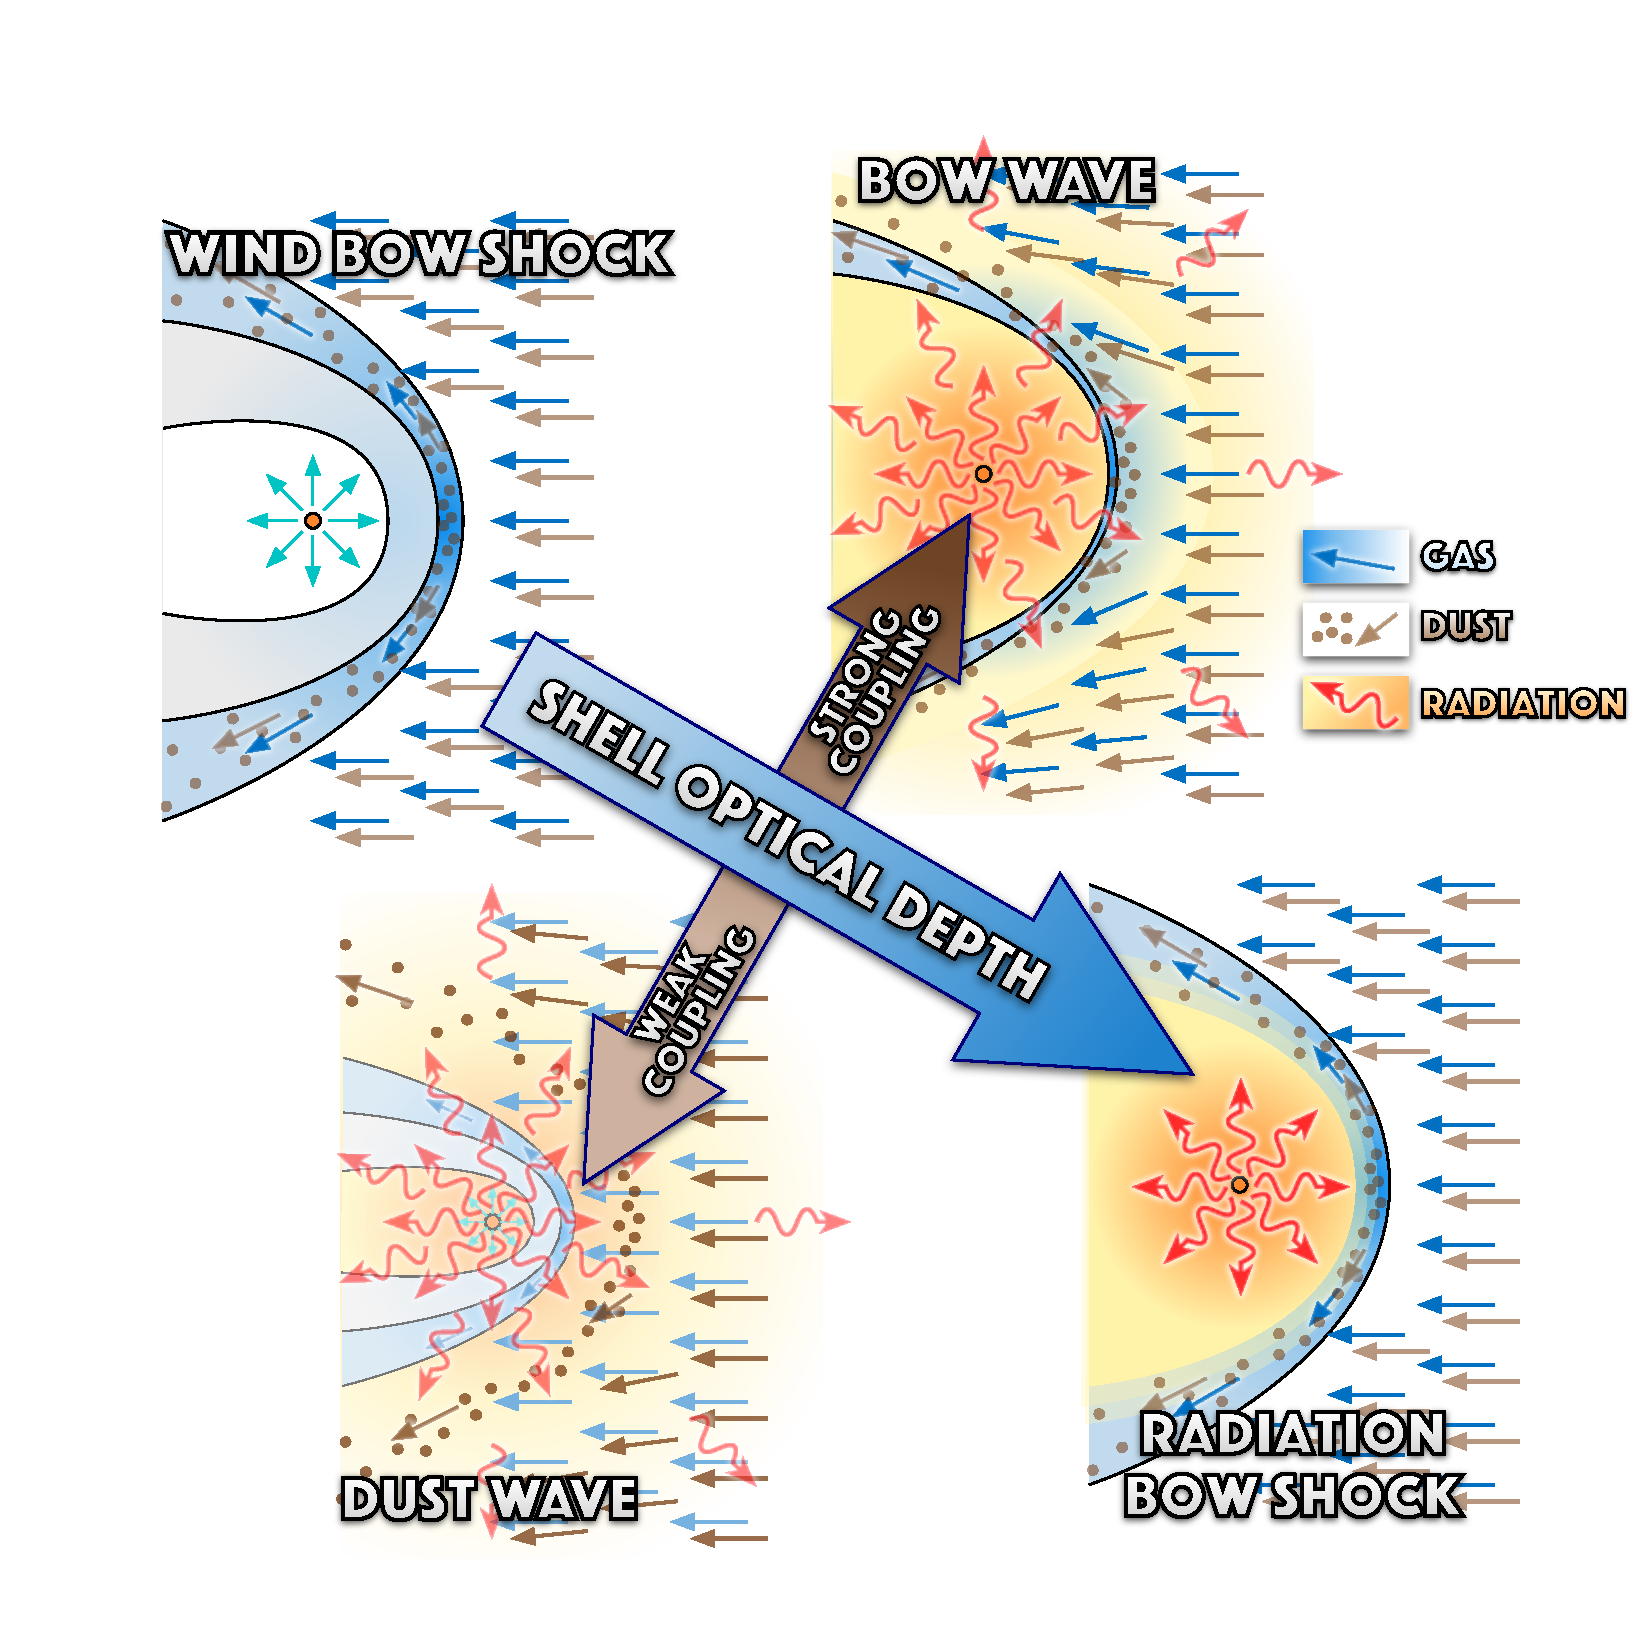
\includegraphics[width=0.8\linewidth]{figs/bows-and-waves}
  \caption{Regimes in the supersonic interaction of a luminous star
    with its environment.  When radiation effects are unimportant, we
    have the standard (magneto-)hydrodynamical wind-supported bow
    shock (upper left), where the ram pressure of the stellar wind
    balances the ram pressure of the oncoming stream.  As the optical
    depth of the shocked shell increases, the stellar radiation
    momentum adds to the wind ram pressure to help support the bow.
    If the shell is completely opaque to stellar radiation, we have a
    radiation-supported bow shock (lower right), where it is the
    stellar radiation pressure that balances the ram pressure of the
    external stream.  For intermediate optical depths, we have two
    cases depending on the strength of coupling between grains and
    gas.  If the coupling is strong, then we have a
    radiation-supported bow wave (upper right), where the plasma
    stream as a whole is gradually radiatively decelerated as it
    approaches the star.  If the coupling is weak, then the radiation
    momentum is felt only by the dust, which decouples from the gas to
    form a dust wave, with the gas stream continuing inward to form a
    wind-supported bow shock closer to the star.  Note that the
    gas--grain coupling is both direct (via collisions) and indirect
    (via the magnetic field) (see Paper~II).}
  \label{fig:3-types-bow}
\end{figure*}

% In \citet[][hereafter \PaperI{}]{Tarango-Yong:2018a}, we proposed a
% new two-dimensional classification scheme for bow shapes: the
% projected planitude--alatude, or \(\Pi'\)--\(\Lambda'\), diagram.  Planitude
% measures the flatness of the bow's apex, while alatude measures the
% openness of the bow's wings.  Both are dimensionless ratios of lengths
% that can be estimated from observational images.  We have analyzed the
% inclination-dependent tracks on the \(\Pi'\)--\(\Lambda'\) plane for simple
% geometric shapes (spheroids, paraboloids, hyperboloids) and for
% thin-shell hydrodynamic bow shock models (wilkinoid, cantoids,
% ancantoids).  In this paper, we will do the same for simple models of
% radiation-driven dust waves (dragoids) and bow waves (trapoids).


This is the first in a series of papers where we develop simple
physical models to show in detail when and how these different
interaction regimes apply when varying the parameters of the star, the
dust grains, and the ambient stream.  We concentrate primarily on the
case of luminous early type stars, where dust is present only in the
ambient stream, and not in the stellar wind.  In this first paper, we
consider the case where the grains are perfectly coupled to the gas
via collisions.  The following two papers consider the decoupling of
grains and gas in a sufficiently strong radiation field
\citep[Paper~II]{Henney:2019b}, and how observations can distinguish
between different classes of bow \citep[Paper~III]{Henney:2019c}.
%
The paper is organized as follows.
%
In \S~\ref{sec:strong-gas-grain} we propose a simple model for stellar
bows and investigate the relative importance of wind and radiation in
providing internal support for the bow shell as a function of the
density and velocity of the ambient stream, and for different types of
star.  In \S~\ref{sec:phys-state-shock} we calculate the physical
state of the bow shell, considering under what circumstances it can
trap within itself the star's ionization front and how efficient
radiative cooling will be.
%
In \S~\ref{sec:summary-discussion} we briefly discuss the application
of our models to observed bows.
%
In \S~\ref{sec:conclusions} we summarise the conclusions of our study. 
%

% In \S~\ref{sec:shape-dust-wave} we do the same for simple models of a
% dusty radiation bow wave (dragoids), including the effects of
% gas-grain drag.
% %
% In \S~\ref{sec:perturbed-bows} we investigate the effects on the
% planitude--alatude plane of small-amplitude perturbations to the bow
% shape.
% %







%%% Local Variables:
%%% mode: latex
%%% TeX-master: "bs-bw-dw-01"
%%% End:
